\documentclass{report}

\usepackage{xcolor}

\usepackage{tikz}
\newcommand*{\tikzgrid}[2]{\draw[help lines](0,0)grid[step=0.2,lightgray,ultra thin](#1,#2);\draw[help lines](0,0)grid[gray](#1,#2);\foreach\x in{0,1,...,#1}\node[below]at(\x,0){\scriptsize\x};\foreach\y in{1,2,...,#2}\node[left]at(0,\y){\scriptsize\y};} 
\usetikzlibrary{arrows.meta}
\usetikzlibrary{shapes.geometric}

\usetikzlibrary{decorations.pathreplacing}

\begin{document}
\chapter{nodos}

	
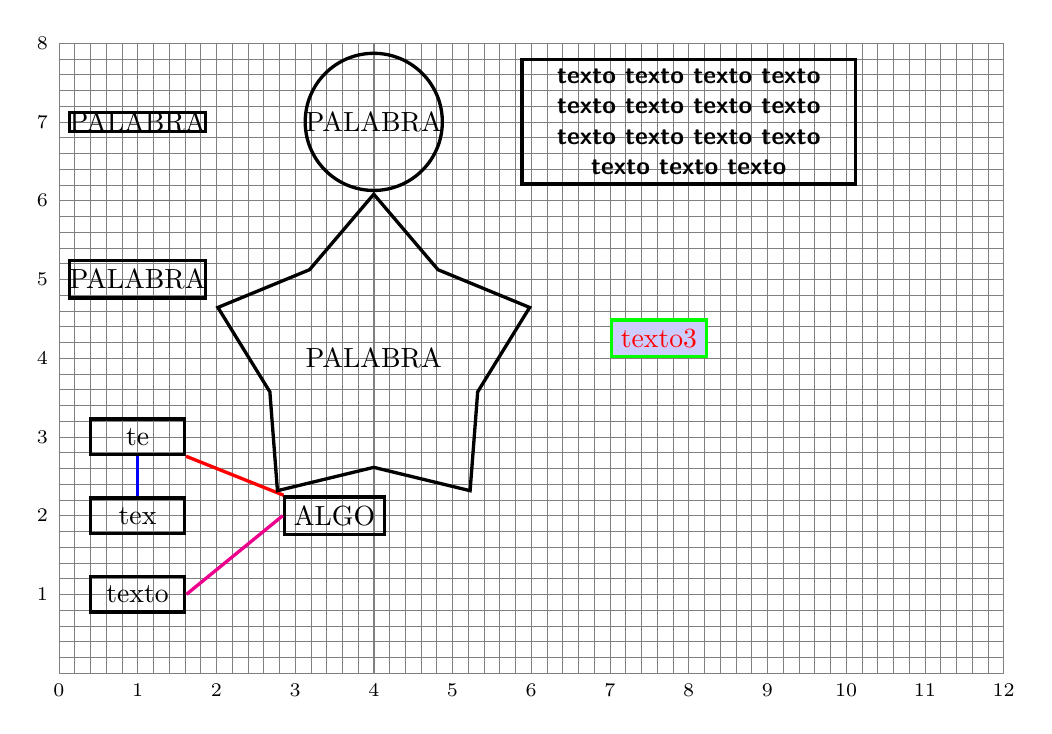
\begin{tikzpicture}[very thick]
\tikzgrid{12}{8}

\node[draw,inner sep=0pt] at(1,7){PALABRA};
\node[draw,inner xsep=0pt] at(1,5){PALABRA};

\node[draw,minimum width=1.2cm](A)at(1,3){te};
\node[draw,minimum width=1.2cm](B)at(1,2){tex};
\node[draw,minimum width=1.2cm](C)at(1,1){texto};
\node[draw](D)at(3.5,2){ALGO};
\draw[blue](A)--(B);
\draw[red](A)--(D);
\draw[magenta](C.0)--(D.180);

\node[draw,inner sep=0pt,shape=circle] at(4,7){PALABRA};
\node[draw,shape=star] at(4,4){PALABRA};

\node[draw,text width=4cm,font=\small\bfseries\sffamily,align=center] at(8,7){ texto texto texto texto texto texto texto texto texto texto texto texto texto texto texto};

\node[draw=green,fill=blue!20,text=red,above right] at(7,4){texto3};

\end{tikzpicture}
	
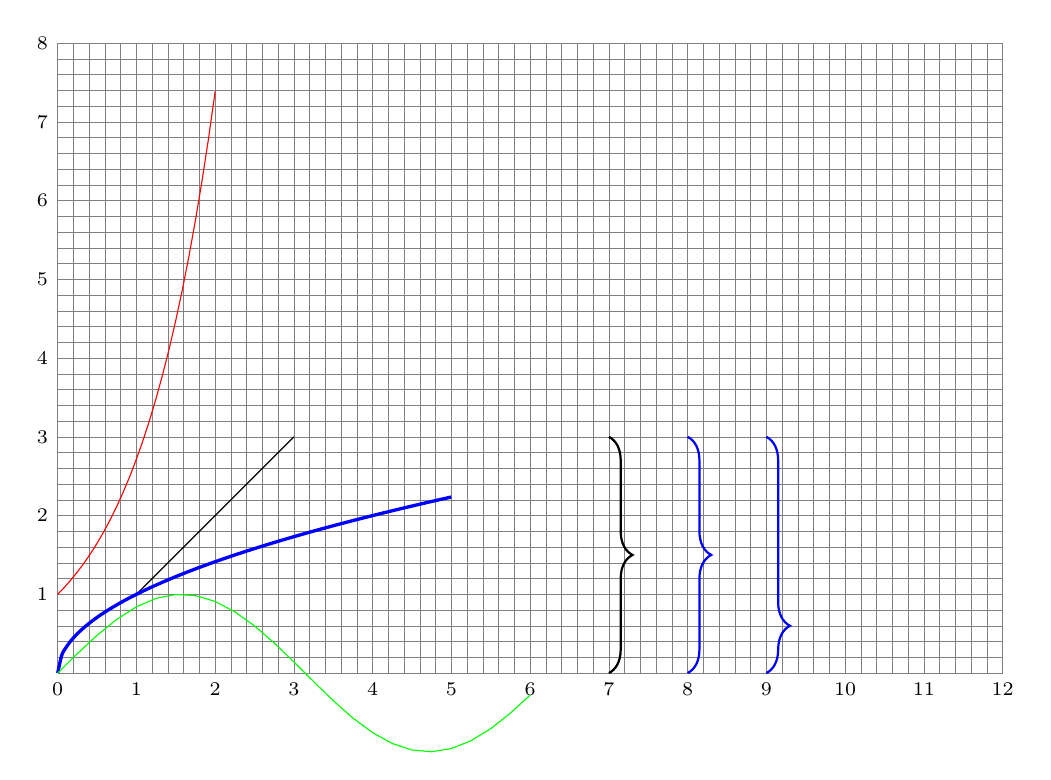
\begin{tikzpicture}
\tikzgrid{12}{8}
\draw(0,0)plot[domain=1:3](\x,\x);
\draw[blue,very thick,smooth](0,0)plot[domain=0:5,samples=100](\x,{sqrt(\x)});
\draw[red](0,0)plot[domain=0:2](\x,{e^(\x)});
\draw[color=green] plot[domain=0:6] (\x,{sin(\x r)});

\draw[thick,decoration={brace,amplitude=3mm},decorate](7,3)--(7,0);

\draw[blue,thick,decoration={brace,amplitude=3mm},decorate](8,3)--(8,0);

\draw[blue,thick,decoration={brace,amplitude=3mm, aspect=0.8},decorate](9,3)--(9,0);
\end{tikzpicture}

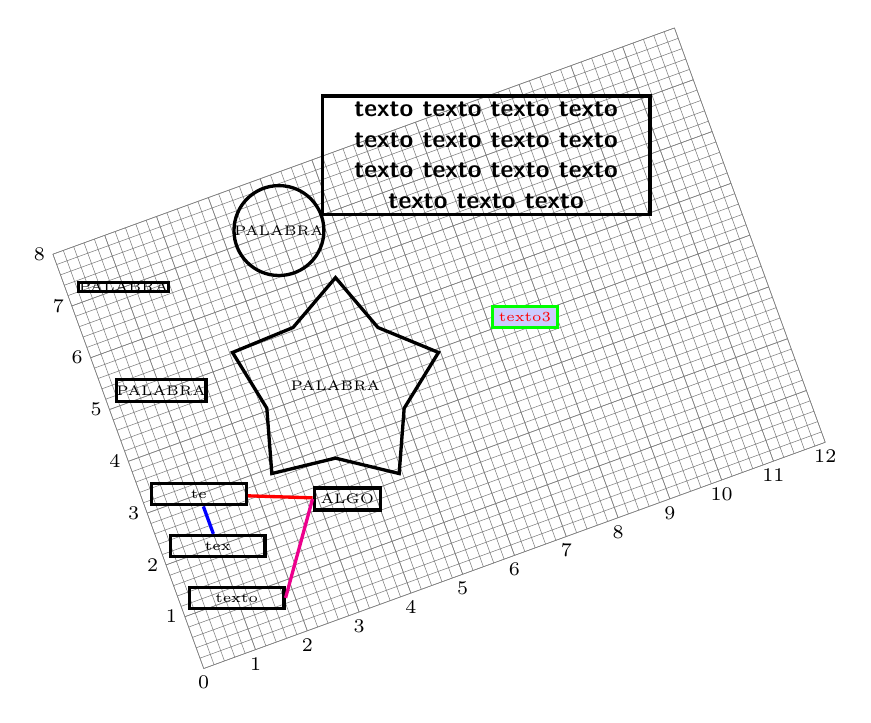
\begin{tikzpicture}[very thick,scale=0.7,rotate=20]\tiny
\tikzgrid{12}{8}

\node[draw,inner sep=0pt] at(1,7){PALABRA};
\node[draw,inner xsep=0pt] at(1,5){PALABRA};

\node[draw,minimum width=1.2cm](A)at(1,3){te};
\node[draw,minimum width=1.2cm](B)at(1,2){tex};
\node[draw,minimum width=1.2cm](C)at(1,1){texto};
\node[draw](D)at(3.5,2){ALGO};
\draw[blue](A)--(B);
\draw[red](A)--(D);
\draw[magenta](C.0)--(D.180);

\node[draw,inner sep=0pt,shape=circle] at(4,7){PALABRA};
\node[draw,shape=star] at(4,4){PALABRA};

\node[draw,text width=4cm,font=\small\bfseries\sffamily,align=center] at(8,7){ texto texto texto texto texto texto texto texto texto texto texto texto texto texto texto};

\node[draw=green,fill=blue!20,text=red,above right] at(7,4){texto3};

\end{tikzpicture}
	
	
\end{document}